\documentclass[aspectratio=169]{beamer}
\usepackage{graphicx}
\usepackage{hyperref}
\usetheme{metropolis}
\title{Graphing (and what not to do)}
\institute{Engineers for Exploration, UC San Diego}
\logo{\includegraphics[height=.65cm,keepaspectratio]{e4e_logo_350x136.png}}
\setbeamertemplate{caption}[numbered]
\begin{document}
\maketitle
\begin{frame}
    What is the purpose of graphs?
\end{frame}
\begin{frame}{Purpose of graphs}
    Visually
    \begin{itemize}
        \item Expressing complex data in a simple format
        \item Illustrate trends/relationships in data
    \end{itemize}
\end{frame}
\begin{frame}{What makes a good graph?}
    \begin{itemize}
        \item Clean, uncluttered look
        \item Label titles, axes, series, and units
        \item Add gridlines to assist with comparison/estimation
        \item Emphasizes key takeaways
        \item Accessible to audience
    \end{itemize}
\end{frame}
\section{Examples of ``bad'' graphs that we've actually seen}
\begin{frame}
    \centering
    \includegraphics[width=\textwidth,height=0.9\textheight,keepaspectratio]{output.png}
\end{frame}
\begin{frame}
    \centering
    \includegraphics[width=\textwidth,height=0.9\textheight,keepaspectratio]{published_archaeology_pie_chart.jpg}
\end{frame}
\begin{frame}
    \centering
    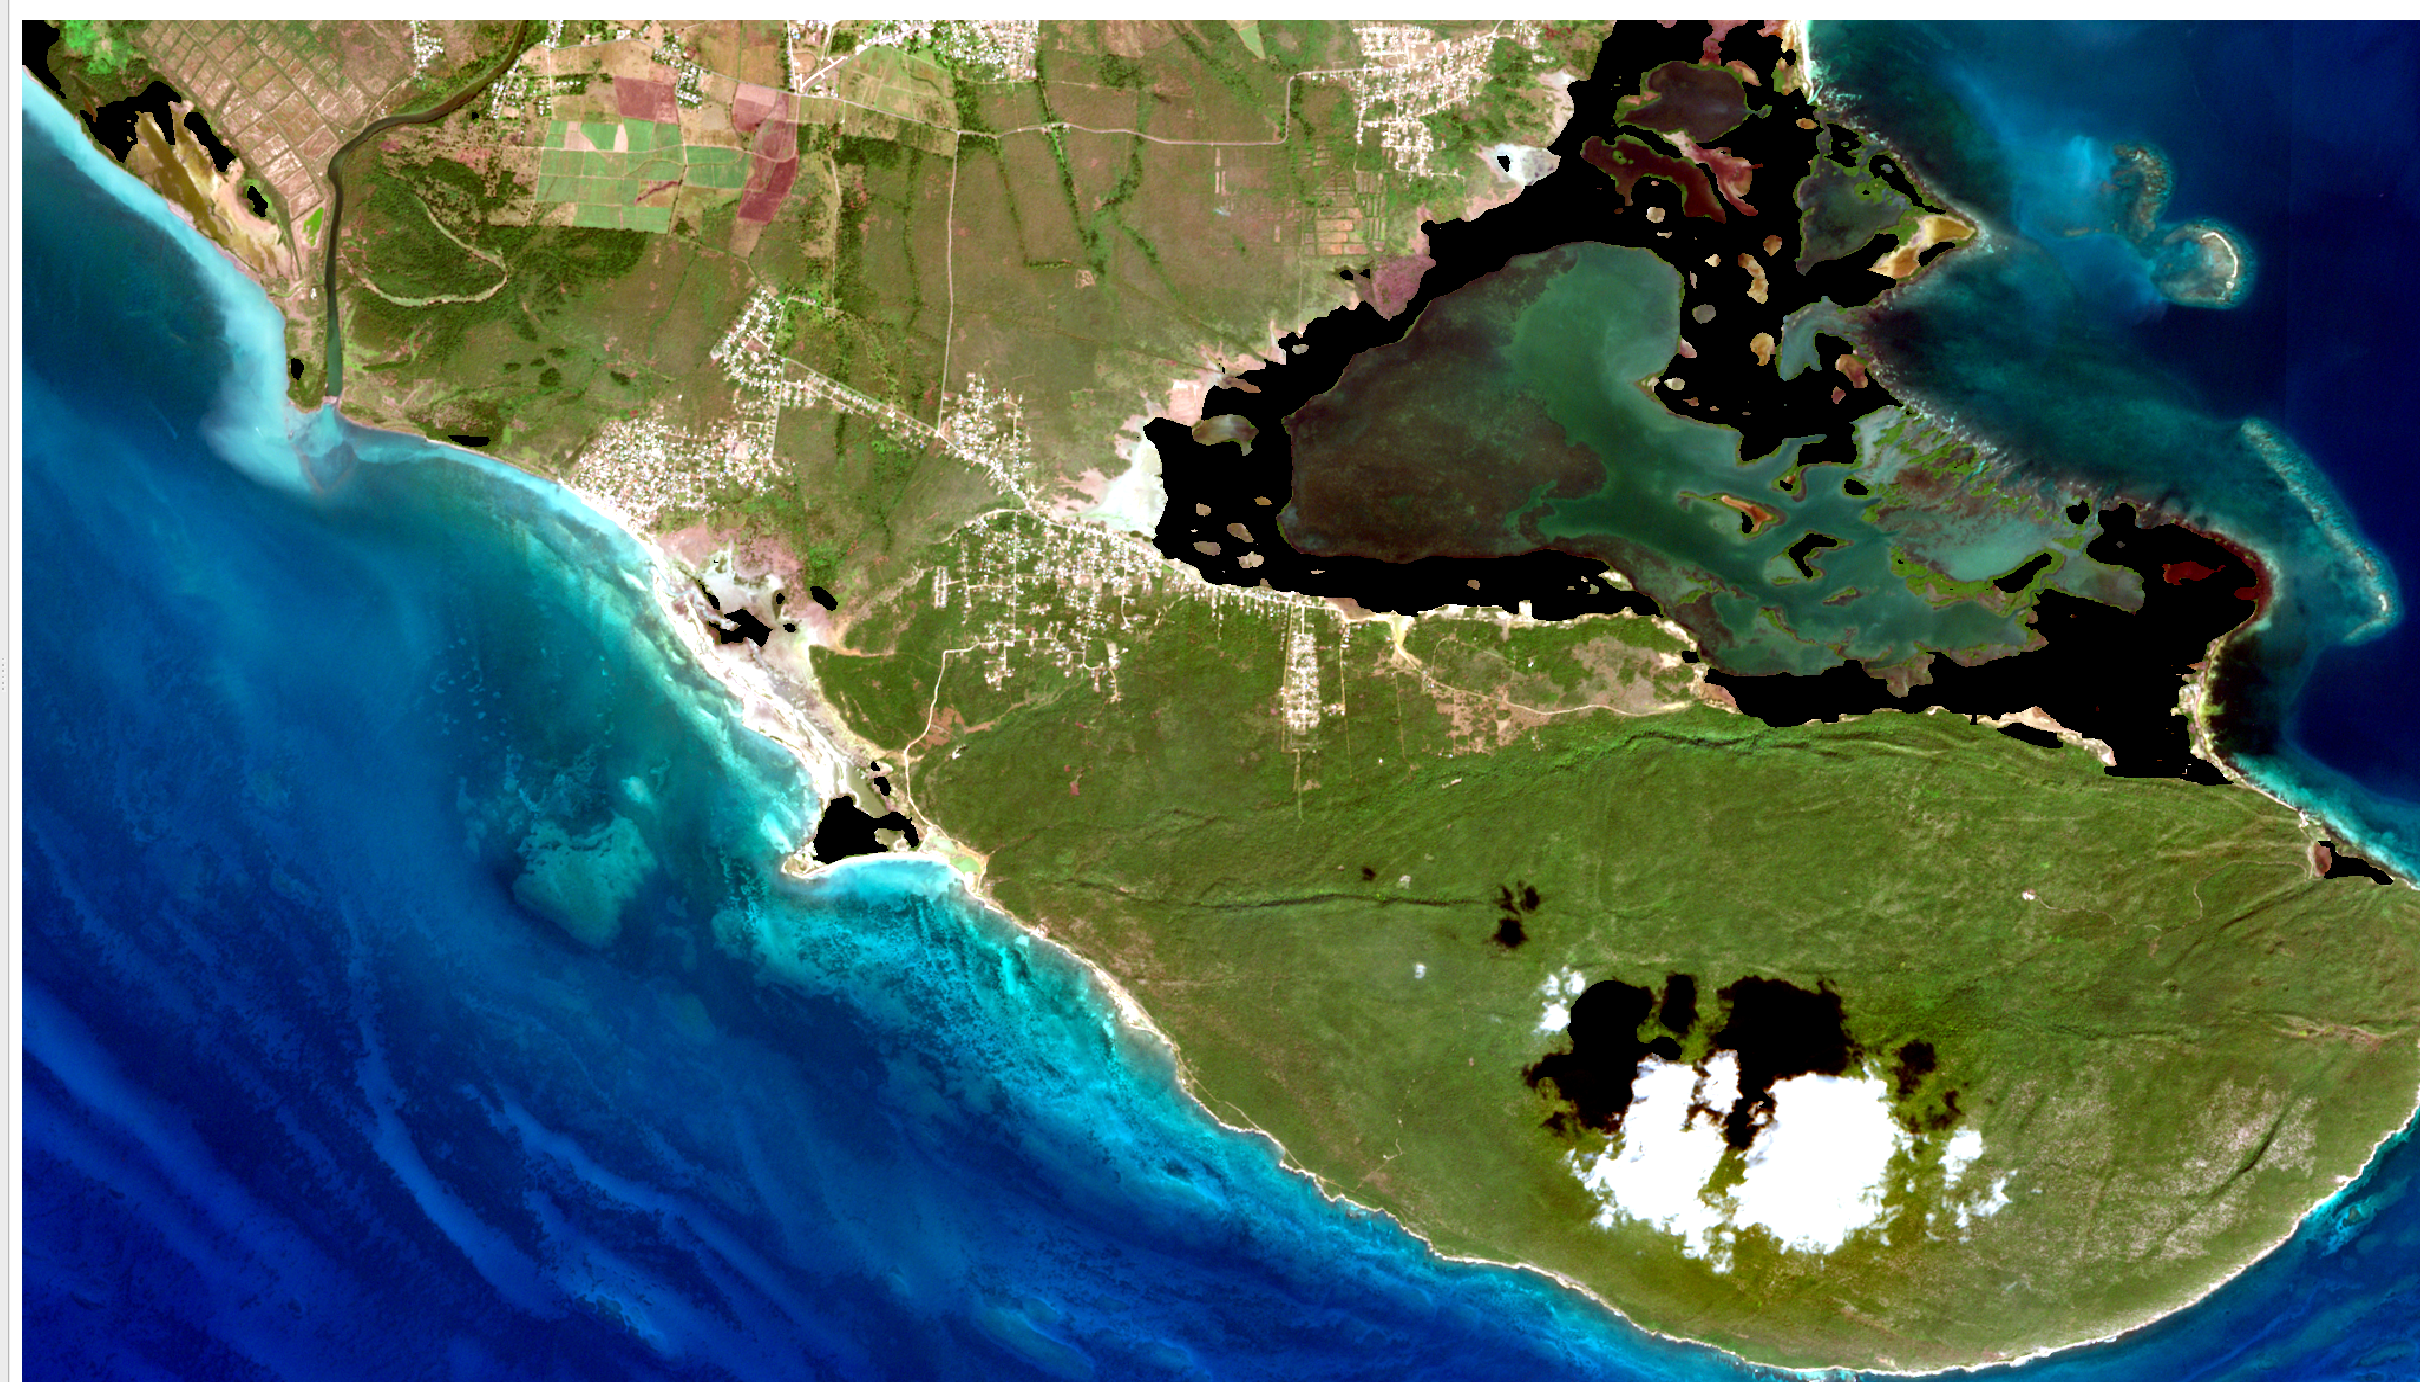
\includegraphics[width=\textwidth,height=0.9\textheight,keepaspectratio]{tiffs.png}
\end{frame}
\begin{frame}
    \centering
    \includegraphics[width=\textwidth,height=0.9\textheight,keepaspectratio]{towerBattery.png}
\end{frame}
\begin{frame}
    \centering
    \includegraphics[width=\textwidth,height=0.9\textheight,keepaspectratio]{XC_conf.png}
\end{frame}
\begin{frame}
    What are some tools you can use to make nice graphs?
\end{frame}
\begin{frame}{What are some tools you can use to make nice graphs?}
    \begin{itemize}
        \item matplotlib
        \item seaborn
        \item bokeh
        \item plotly
        \item pandas
    \end{itemize}
\end{frame}
\begin{frame}{Ways to make plotting easier}
    \begin{itemize}
        \item Use Jupyter notebooks
        \item Separate data processing and visualization
        \item Save intermediate data
        \item Save final figures to disk (png/svg)
        \item Do all of the resizing/rendering in the chart generation
    \end{itemize}
\end{frame}
\end{document}